\documentclass[11pt, oneside]{article} 
\usepackage{geometry}
\geometry{letterpaper} 
\usepackage{graphicx}
	
\usepackage{amssymb}
\usepackage{amsmath}
\usepackage{parskip}
\usepackage{color}
\usepackage{hyperref}

\graphicspath{{/Users/telliott_admin/Dropbox/Tex/png/}}
% \begin{center} 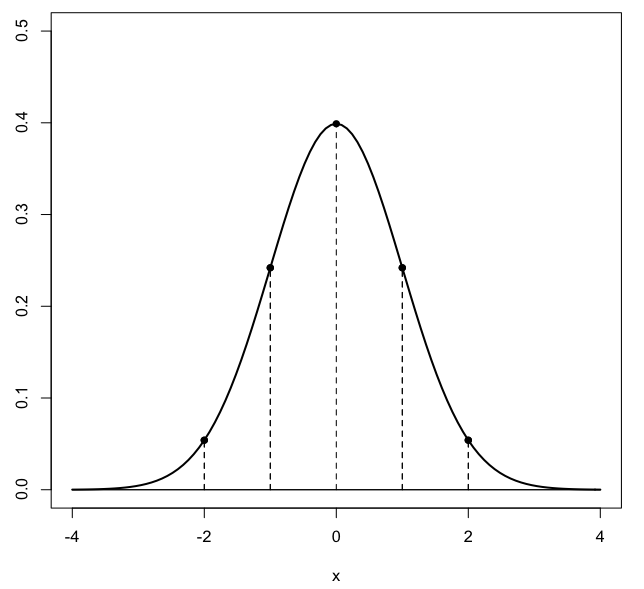
\includegraphics [scale=0.4] {gauss3.png} \end{center}

\title{Galois fields}
\date{}

\begin{document}
\maketitle
\Large
Finite fields are called Galois fields, honoring Galois, and often given a name such as GF($7$) or GF($2^8$).  The wikipedia article on finite fields is pretty dense, as is typical for math topics there.

\url{https://en.wikipedia.org/wiki/Finite_field}

This short set of chapters is an exploration of Galois fields as they relate to cryptography in AES, the advanced encryption standard.  Galois field theory is a famously complex subject, and I don't pretend to understand it.  

However, I have worked carefully through the bits of it that relate to AES, and written it here.

Wikipedia:

\begin{quote}As with any field, a finite field is a set on which the operations of multiplication, addition, subtraction and division are defined and satisfy certain basic rules. The most common examples of finite fields are given by the integers mod p when p is a prime number.\end{quote}

One of my better sources is

\url{https://engineering.purdue.edu/kak/compsec/Lectures.html}

I'll start with some notes on early chapters from Prof. Kak's course on cryptography.

\section*{Definitions}

\subsection*{Group}

A \textbf{group} is a set of objects plus a binary operation.  The binary operator may be given a generic symbol like $o$, but a common notation is to use \{G,+\}, (even if the operation is not really like addition). 

Properties:  if a,b $\in$ G, then the operations exhibit:
\begin{itemize}
\item Closure:           $a \ + \ b = c$ $\Rightarrow$ c $\in$ G
\item Associativity:    $(a \ + \ b) \ + \ c = a \ + \ (b \ + \ c)$
\item Identity element:  $a \ + \ i = a$
\item Inverse element:   $a \ + \ b = i$
\end{itemize}

Groups are about \emph{addition}, for some suitable definition of addition.

Typically $0$ is used for the identity element ($a + 0 = a$).

Commutativity is not necessarily a property of a group.

\begin{itemize}
\item Commutative:       $a \ + \ b = b \ + \ a$
\end{itemize}

If a group is commutative it is called an \textbf{Abelian group}.

\subsection*{Ring}
A \textbf{Ring} is a group which also has the multiplication operator $\times$ (even if the operation is not really like multiplication).  It may be designated as \{R,+,$\times$\} and has the following properties:

\begin{itemize}
\item Closure:           $a \times b \in R$
\item Associativity:     $(a \times b) \times c = a \times (b \times c)$
\item Distributivity:    $a \times (b + c) = (a \times c) + (a \times b)$
\end{itemize}

Repeating from the group definition, for rings we see closure and associativity \emph{under} multiplication.  Since there are two operations we can order them in different ways, hence the example for distributivity.

Notation:  often the $\times$ is dropped:  $a(b + c) = ac + ab$.  

As with groups, a ring  \emph{may} be 
\begin{itemize}
\item Commutative:    $ab = ba$
\end{itemize}

An \textbf{integral domain} \{R,+,$\times$\} is a commutative ring that also has a
\begin{itemize}
\item Multiplicative identity element:    $a \times 1 = a$
\end{itemize}

If $ab = 0$, then either $a = 0$ or $b = 0$.

\subsection*{Field}
A field has all of the above properties.  It is an integral domain.  

And for every $a$, there exists a $b$ such that

\begin{itemize}
\item Multiplicative inverse:   $ab = 1$
\end{itemize}

$1$ is its own multiplicative inverse.

According to wikipedia

\url{https://en.wikipedia.org/wiki/Finite_field}

\begin{quote}In mathematics, a finite field or Galois field ... is a field that contains a finite number of elements. As with any field, a finite field is a set on which the operations of multiplication, addition, subtraction and division are defined and satisfy certain basic rules.\end{quote}

You can read all about it there.  I \emph{think} this conveys the general idea.

\subsection*{Operations}

At this point we talk (briefly) about the special operations used for the Galois fields in cryptography.  

"Addition" is defined as "exclusive or", XOR, often symbolized $\oplus$.  

For binary numbers
\[ 0 \oplus 0 = 1 \oplus 1 = 0, \ \ \ \ 1 \oplus 0 = 0 \oplus 1 = 1 \]
\[ 0011 \oplus 0101 = 0110 \]
It is perhaps easier to see if they are lined up properly
\begin{verbatim}
0011
0101
----
0110
\end{verbatim}

Two points:
\begin{itemize}
    \item{binary numbers $> 1$ can be used}
    \item{$x \oplus y = z \rightarrow x \oplus z = y$ and $z \oplus y = x$}
\end{itemize}

Python has an XOR for decimal numbers:
\begin{verbatim}
>>> 23 ^ 17
6
>>>
\end{verbatim}

Explanation:
\begin{verbatim}
10111 = 23
10001 = 17
------
00110 = 6
\end{verbatim}

This \emph{not} addition, there is no carry.

We'll talk about multiplication in a later part.  The next chapter is about modular arithmetic.

\end{document}